\subsection{Horizontal velocity (glacier flow)}

\begin{figure}[H]
    \centering
    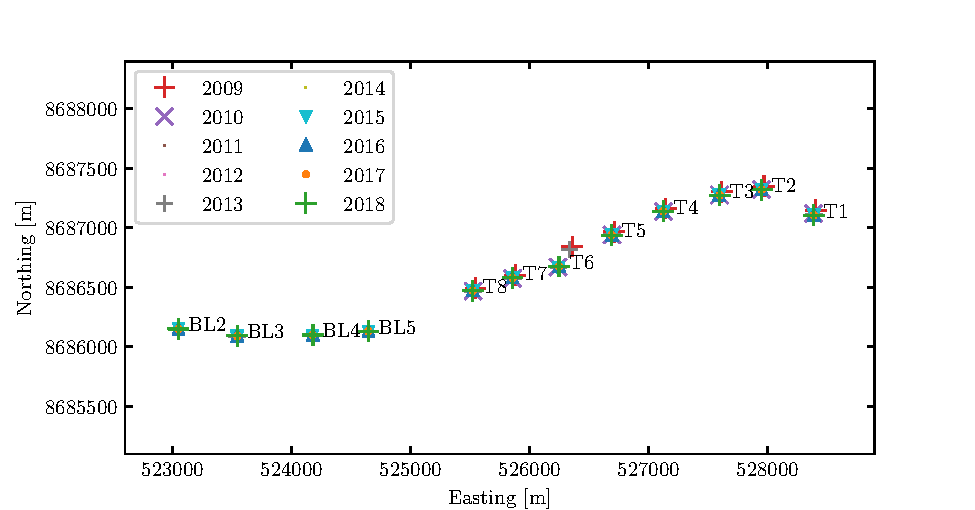
\includegraphics[width=\textwidth]{./figs/stakePositions.pdf}
    \caption{Positions of all stakes in the flow line on Blekumbreen and Tellbreen.
    The different markers distinguish the year of the measurement.}
    \label{GF:fig:stakepos}
\end{figure}






\begin{table}[h]
	\caption{Velocity of the stakes measured in 2018, calculated with equations~\ref{GF:eq:v} and \ref{GF:eq:sv}.
	The velocity of all stakes has been calculated using last years position.
	If available, positions from 2016 and 2015 have also been used.}
	\centering
	%\scriptsize
	\begin{tabular}{lcccccc}
\toprule
  Stake name & Velocity (2017) [m/a] & Velocity (2016) [m/a] & Velocity (2015) [m/a] \\
\midrule
    BL2-2016 &       0.26 $\pm$ 0.21 &       0.21 $\pm$ 0.20 &                     - \\
    BL3-2016 &       0.16 $\pm$ 0.20 &       0.21 $\pm$ 0.18 &                     - \\
  BL4-i-2016 &       0.07 $\pm$ 0.26 &       0.08 $\pm$ 0.25 &                     - \\
 BL4-ii-2016 &       0.11 $\pm$ 0.56 &       0.05 $\pm$ 0.48 &                     - \\
  BL5-i-2017 &       1.75 $\pm$ 0.18 &                     - &                     - \\
 BL5-ii-2017 &       1.74 $\pm$ 0.24 &                     - &                     - \\
   T1-i-2017 &       0.09 $\pm$ 0.11 &                     - &                     - \\
  T1-ii-2017 &       0.19 $\pm$ 0.43 &                     - &                     - \\
     T2-2016 &       0.60 $\pm$ 0.24 &       0.28 $\pm$ 0.20 &                     - \\
   T2-i-2017 &       0.23 $\pm$ 0.30 &                     - &                     - \\
  T2-ii-2017 &       0.53 $\pm$ 0.51 &                     - &                     - \\
     T3-2017 &       0.10 $\pm$ 0.12 &                     - &                     - \\
     T4-2016 &       0.13 $\pm$ 0.38 &       0.17 $\pm$ 0.37 &                     - \\
     T5-2016 &       0.30 $\pm$ 0.33 &       0.12 $\pm$ 0.22 &                     - \\
     T6-2016 &       0.79 $\pm$ 0.31 &       0.12 $\pm$ 0.19 &                     - \\
     T7-2015 &       0.26 $\pm$ 0.27 &       0.10 $\pm$ 0.15 &       0.08 $\pm$ 0.19 \\
     T7-2017 &       1.33 $\pm$ 0.16 &                     - &                     - \\
     T8-2017 &       0.20 $\pm$ 0.24 &                     - &                     - \\
\bottomrule
\end{tabular}

	\label{GPS:tab:os_tab}
\end{table}

\begin{equation}
\label{GF:eq:v}
v = \frac{\sqrt{(N_{2018}-N_{ref,year})^2+(E_{2018} - E_{ref,year})^2}}{t}
\end{equation}

\begin{equation}
\label{GF:eq:sv}
s_v = \sqrt{\frac{(\delta_{N_{2018}}^2 + \delta_{N_{ref,year}}^2) * (N_{2018}-N_{ref,year})^2 +
(\delta_{E_{2018}}^2 + \delta_{E_{ref,year}}^2) * (E_{2018}-E_{\text{ref,year}})^2}
{(N_{2018} - N_{ref,year})^2+ (E_{2018} - E_{ref,year})^2}}
\end{equation}

\begin{figure}[H]
    \centering
    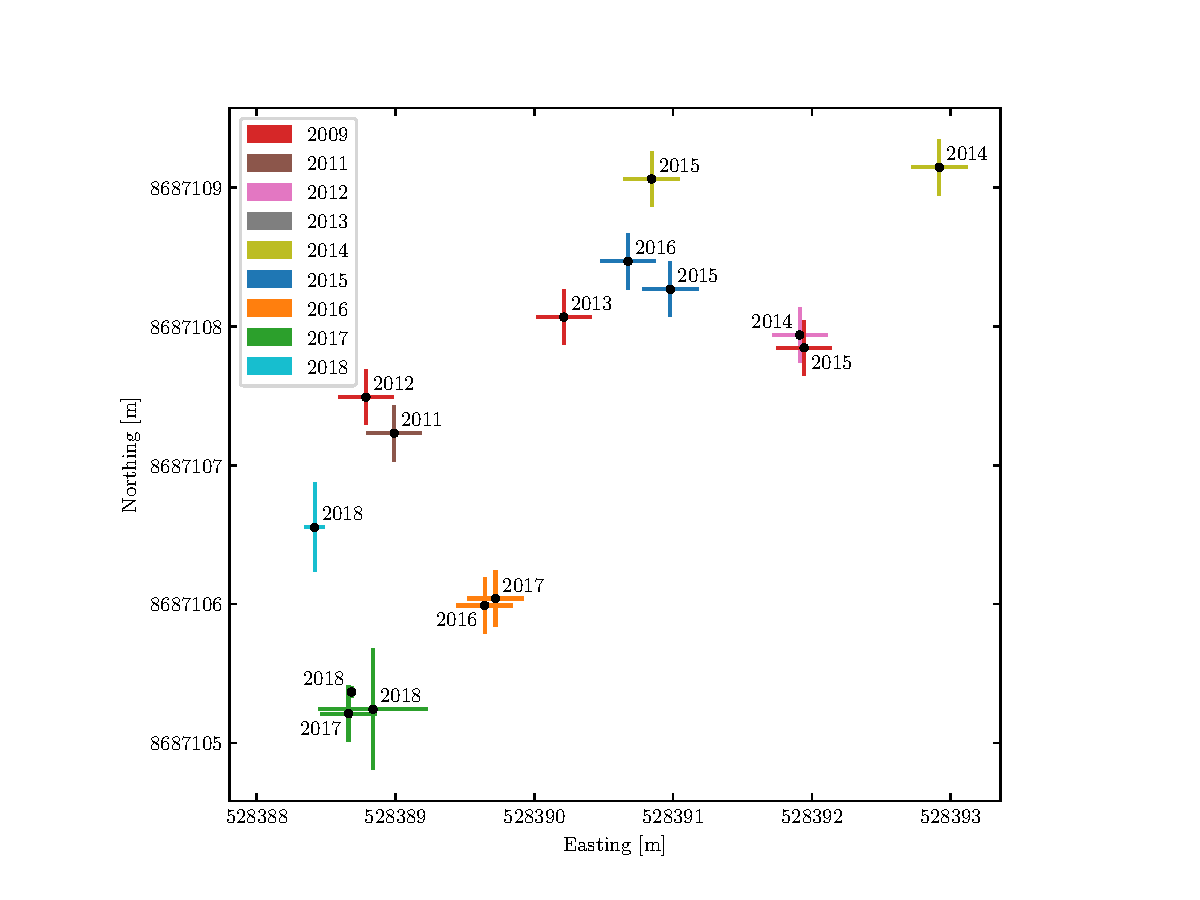
\includegraphics[width=\textwidth]{./figs/T1_2d.pdf}
    \caption{Measured position of stake T1 from 2009 to 2017.}
    \label{GF:fig:T1_2d}
\end{figure}


\subsection{Vertical velocity (mass balance)}